\documentclass[a4paper, oneside]{memoir}% Document class
\usepackage[a4paper]{geometry}			% Margins
\usepackage{lmodern}
\usepackage{graphicx}
\usepackage{float}
\usepackage{listings}
\usepackage[small,compact]{titlesec}	% No 'chapter' in chapter headings.
\graphicspath{{Media/}}					% Directory that holds images.

\titleformat{\chapter}[hang]
{\normalfont\Large\bfseries}{\thechapter}{1em}{\Large}
\titlespacing{\chapter}{0pt}{*0}{*1}

\titleformat{\chapter}{\Huge\bfseries}{\thechapter}{1em}{}
\titleformat{\section}{\LARGE\bfseries}{\thesection}{1em}{}
\titleformat{\subsection}{\Large\bfseries}{\thesubsection}{1em}{}
\titleformat{\subsubsection}{\normalsize\bfseries}{\thesubsubsection}{1em}{}


\author{
  Erik Sidelmann Jensen\\
  \texttt{ejens11@student.aau.dk}
  \and
  Lasse Vang Gravesen\\
  \texttt{lgrave11@student.aau.dk}
  \and
  Dennis Jakobsen\\
  \texttt{djakob11@student.aau.dk}  
}

\title{Web Intelligence - Crawler Miniproject}
\date{}

\begin{document}
	\clearpage\maketitle
	\thispagestyle{empty}
	
	\chapter{Crawler Miniproject}
	\section{Crawler}
	The crawler retrieves the documents used for the search engine, it starts by using a list of seed urls.
	The seed site for ours was \url{http://en.wikipedia.org/wiki/Internet_of_Things}.
	Politeness was important, in that the crawler had to adhere to the `robots.txt' file on websites and determine if the crawler was allowed to visit the url in question and at the same time the crawler should not visit a page too often, this was implemented by simply just waiting a second after each visit. 
	Equality of content on pages had to be checked because there is no reason to have multiple pages with the same content in the search results, we did this using sketches with Shingling and Jaccard similarity. The general idea of shingling can be demonstrated using the following string: "This is a string", with a shingle size of 2, the resulting shingles would be "This is", "is a", "a string". These can then be used to check equality against a different document using the aforementioned Jaccard similarity. 
	
	$$ J(A,B) = \frac{| A \cap B |}{|A \cup B|} $$
	
	The Jaccard similarity is then some value between 0 and 1, and if it is above the threshold, say 0.9, the two documents are said to be equal.
	
	Sketching is then when you use multiple hashing functions on the shingles and get the minimum hashed shingle for each hashing function, and then run jaccard similarity on those.
	
	The crawler also needs to extract urls from the document, it does this using a regular expression. To simplify the regular expression we only get the urls inside an href attribute. These urls then are normalized, fixed and added to the frontier if they have not already been visited or they are not in the frontier already.
	
	The architecture is somewhat similar to the architecture shown in the slides, though there are some differences specifically with the `robots.txt' check in that it does that check for each url it visits instead of performing the check before adding it to the frontier. See \figref{fig:basiccrawlarchitecture}.
	
	\begin{figure}[H]
	\centering
	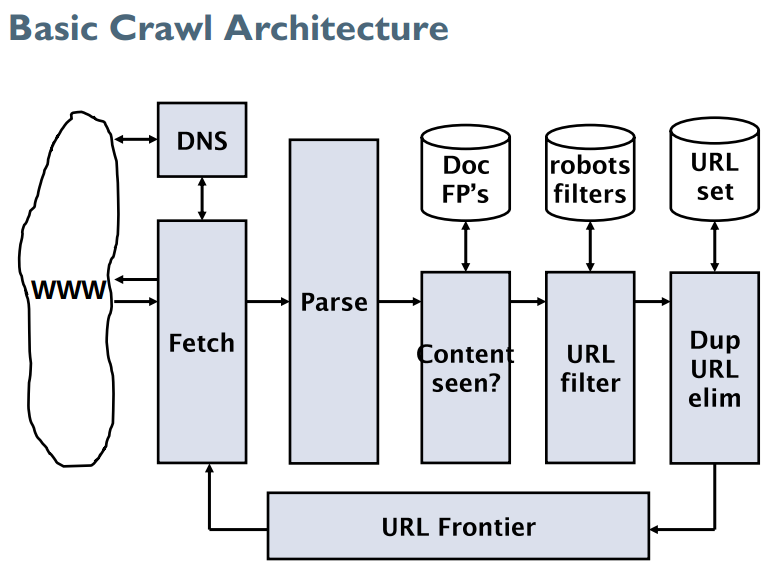
\includegraphics[width=0.7\linewidth]{./Media/basiccrawlarchitecture}
	\caption{Basic Crawl Architecture from Slides}
	\label{fig:basiccrawlarchitecture}
	\end{figure}
	
	To sum up: It gets an url from the frontier, fetches the content if it can get past the `robots.txt' checker, parses out the word content and checks if that has already been seen, and adds it to the url filter after normalizing and checking if it does not already exist in the frontier or already visited urls.
	
	\subsection{Cut Corners}
	The Crawler does not find every url in the visited urls, but rather just the ones that are inside href attribute.
	
	The Crawler was limited to very few pages, 100-1000 because waiting a second after each page is limiting.
	
	The sketches for each document is kept in memory.
	
	\section{Indexer}
	The purpose of the indexer is to sort through the crawled documents, and create something that can be easily utilized by the search engine. It does this by providing an inverted index of the terms and which documents contain them and their frequency in said documents.
	We use an inverted index because then we do not need to investigate every document for matches but rather we can just look at the individual terms and see what documents match.
	The indexer works by retrieving the crawled pages in the database as an object that contains the html document, the url and the document id.
	The html document is converted into only words and these are tokenized by splitting them. 
	These words are made into features, by stemming them using an English language stemmer. It also removes the English stopwords, such as "the" or "a".
	It is important to note that the query gets the same treatment, in that it is tokenized, stemmed and that the stopwords are removed because if you do not do that the terms in the inverted index will not match.
	That feature(or term) is then added to the inverted index along with the id of the document.
	
	Adding to the inverted index works as such, it receives the term and the document id as mentioned, checks if the inverted index already contains the term.
	
	If the inverted index does not already contain the term, it creates a list of postings, adds a posting with the document id, and adds that to inverted index using the term and a new posting list.
	
	If the inverted index does contain it, it checks if the document id already has a posting because we might encounter the same word multiple times in the same document. It then sorts the postings.
	
	Otherwise it increments the term frequency of that term for the current document.
	
	The structure of the inverted index can be seen in \figref{fig:InvertedIndex}.
	
	\begin{figure}[H]
	\centering
	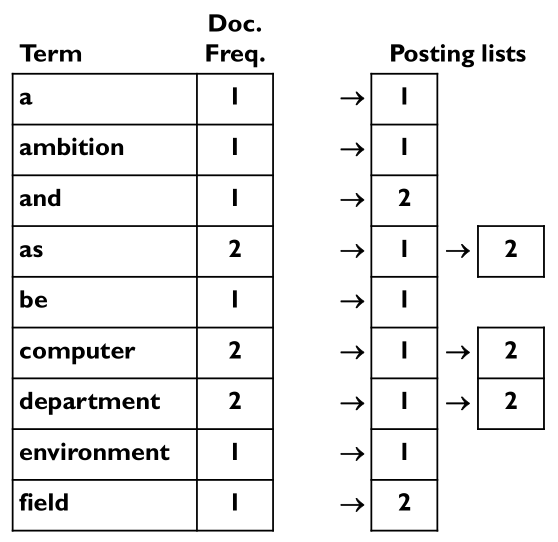
\includegraphics[width=0.7\linewidth]{./Media/InvertedIndex}
	\caption{The inverted index. Source: From the Lecture 3 slides page 36.}
	\label{fig:InvertedIndex}
	\end{figure}
	
	This inverted index is kept in memory.
	
	The general idea of what the indexer does can be seen in \figref{fig:indexer}.
	
	\begin{figure}[H]
	\centering
	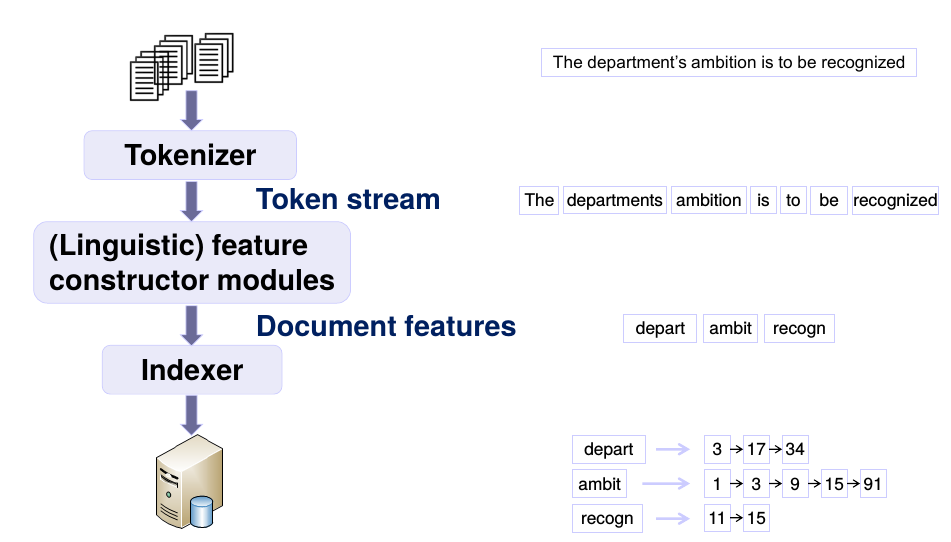
\includegraphics[width=0.7\linewidth]{./Media/indexer}
	\caption{Indexer. Source: From the Lecture 3 slides page 7.}
	\label{fig:indexer}
	\end{figure}
	
	\section{Ranker}
	The purpose of the ranker is to get the most relevant results for the user given some query.
	For the ranker we used the cosine score algorithm based on tf-idf weighting.
	The cosine score algorithm uses cosine similarity between the angle of tf-idf vectors.
	
	The general idea behind that can be seen in \figref{fig:CosineSimilarity}
	
	\begin{figure}[H]
	\centering
	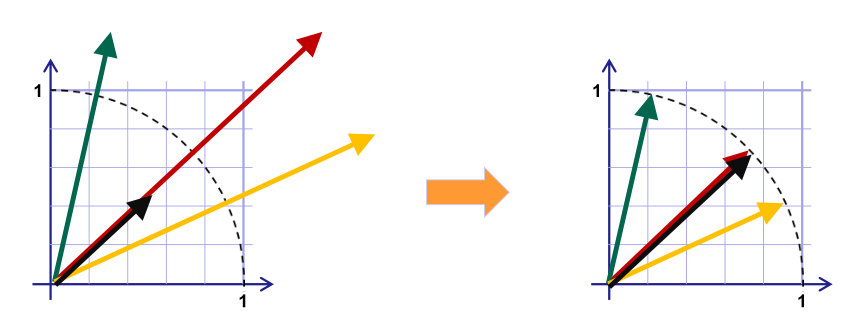
\includegraphics[width=0.7\linewidth]{Media/CosineSimilarity}
	\caption{The idea behind cosine similarity. Source: From the Lecture 4 slides page 32.}
	\label{fig:CosineSimilarity}
	\end{figure}
	
	What the ranker does specifically is that it takes a query, tokenizes it and constructs features using the stemmer and stopword removal because the query needs to be treated the same way as the documents were in the indexer.
	
	The tf(Term Frequency) weight is the amount of times a document contains a term.
	
	The tf* weight is $$log_{10}(1+tf_{t,d})$$ because relevance does not increase proportionally we need to log10 it.
	
	The df(Document Frequency) weight is the amount of times a term is mentioned in all the documents.
	
	The idf(Inverse Document Frequency) weight is $$log_{10}(\frac{N}{df_{t}})$$ where N is the total amount of documents.
	
	The tf-idf weight is then $$tf*idf$$
	
	Using tf-idf we can then calculate a score for each document using the cosine score algorithm mentioned previously, and this is then used to sort the results and provide a good output for the user, for example ~10 documents.
	
	tf-idf weighting has different variants, like ltc or lnc. The one we use is ltc.
	
	We also implemented contender pruning using 'Champions Lists' where you precompute for each term t, r amount of docs of the highest weight(the tf weight) and this list is then looked at first instead of the default list of postings as a champion list.
	
	All this comes together to form a search engine, which can be seen in \figref{fig:searchenginearchitecture}
	
	\begin{figure}[H]
	\centering
	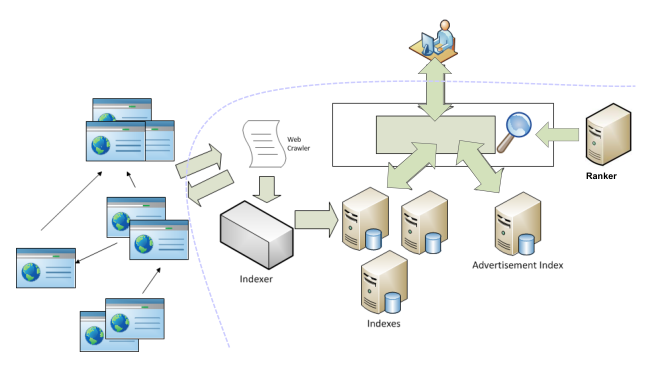
\includegraphics[width=0.7\linewidth]{Media/searchenginearchitecture}
	\caption{Search Engine Architecture. Source: From the Lecture 1 slides page 27.}
	\label{fig:searchenginearchitecture}
	\end{figure}

\end{document}
